%---------------------------------------------------------------------------------------------------
%		introduction.tex
%
%	This is file contains an introduction about the SOA architectural desing.
%
%	Author: Andrea Meneghinello
% Version: 0.1
%	Table of changes:
%		21/03/2016 -> document definition
%---------------------------------------------------------------------------------------------------
\section{\acs{soa} re-visitation}
\label{sec:architecture-soaRevisitation}
In the following section we want to review the \ac{soa} architecture in order to exploit its main
characteristics. We will use the re-visitation later in our architecture in order to provide an
elastic and multi-tenant architecture deployable in the \ac{paas}.

\subsection{\acf{soa}}
A \acf{soa} is an architectural model for the creation of systems that reside over a network and
focus their attention over the concept of \keyword{services}. A system built following the \ac{soa}
philosophy is made of applications called services. They are well defined, independent from each
other and they can reside on multiple computers linked in a network.

Each service makes a certain functionality available, and can utilize the ones made available by other
services. Though this architecture, we are able to build more sophisticated applications starting from
elementary components. Its work model is illustrated in Figure \ref{img:architecture-soaRevisitation-workmodel}

\begin{figure}
	\centering{}
	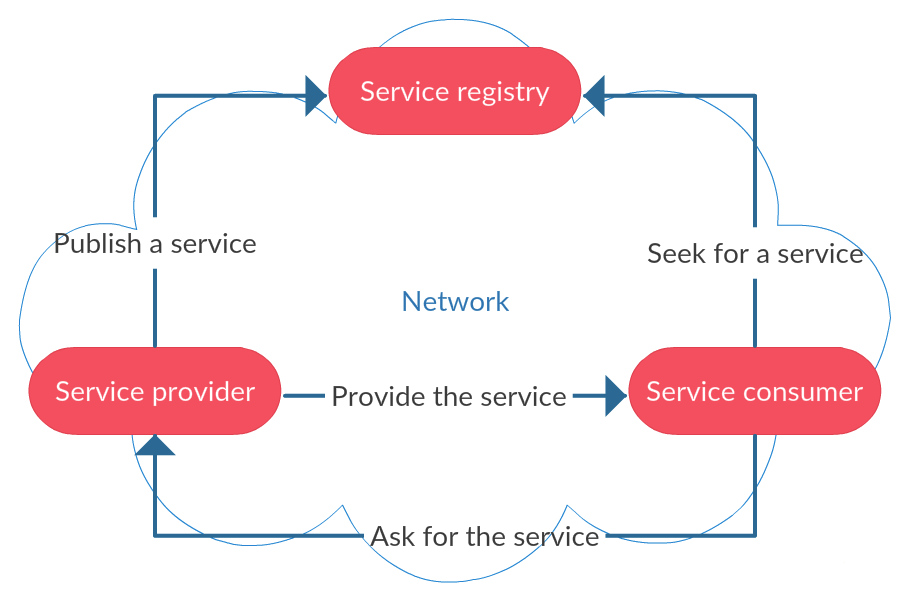
\includegraphics[width=0.7\textwidth]{chapters/architecture/images/soa-workmodel.png}
	\caption[Example of \acs{soa} architecture]{Example of \acf{soa} architecture.}
	\label{img:architecture-soaRevisitation-workmodel}
\end{figure} 

\ac{soa} abstraction is not related to any specific technology, but it simply defines some properties 
that are oriented to the \keyword{reuse} and to the \keyword{integration} in a heterogeneous environments
of its base components.

In particular, each service must have the following properties (illustrated in Figure 
\ref{img:architecture-soaRevisitation-characteristics}):

\begin{itemize}
	\item{\keyword{service discoverability}: a service must be retrieved basing on its interface and
		called at run-time;}
	\item{\keyword{service autonomy}: every service must be well defined, complete and independent
		from the context or from the status of other services;}
	\item{\keyword{standardized service contract} and \keyword{service abstraction}: services must
		be defined in terms of what they do, abstracting them from the technologies used to implement
		them. This determines the independence from both the used programming language and the \acs{os}
		on which they are running. It is not necessary to know how a service is implemented but only
		the offered functionalities.}
	\item{\keyword{service loose coupling}: an architecture is loosely coupled if the dependencies
		between its components are limited. Thus, we have to made services that depends least as possible
		by other making the system flexible and easily customizable;}
	\item{\keyword{service reusability}: each service must be made available on the network through
		the publication of its interface and made accessible in a transparent way (location awareness);}
	\item{\keyword{service statelessness}: the services minimize the resource consumption and delegate
		the status information management when necessary;}
	\item{\keyword{service composability}: in a \ac{soa} architecture the applications are the result of
		the composition of many services. This is the reason that leads us to build independent services
		in order to obtain the maximum re-usability. The creation of applications or more complex
		services through composability is defined as \keyword{service orchestration}.}
\end{itemize}

\begin{figure}
	\centering{}
	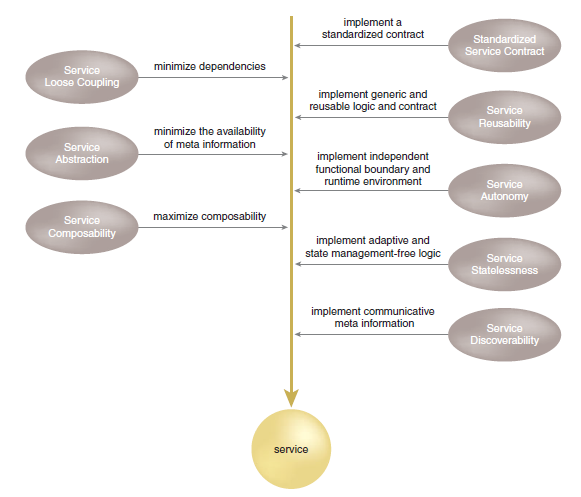
\includegraphics[width=0.7\textwidth]{chapters/architecture/images/soa-characteristics.png}
	\caption[Service oriented logic]{Service oriented logic \cite{serviceCharacteristics}.}
	\label{img:architecture-soaRevisitation-characteristics}
\end{figure}

\subsubsection{Difference with cloud computing model}
\label{sec:architecture-soaRevisitation-compatibility}
\ac{soa} architecture was born in the pre-cloud era, thus it is not conceived to address cloud computing
issues. But \ac{caa} and \ac{soa} share some characteristics that bring us to consider \ac{soa}'s base
philosophy while building our architecture.

First, both emphasize the \keyword{service concept}. By definition, a service is made up by smaller parts
that do the job to build the final output, everyone use the \keyword{delegation} system. With that methodology,
people can use the services without worrying about their implementation details and their scalability. In
addiction, services can be shared by multiple applications and users, thus optimizing resource consumption,
and enabling the concept of multi-tenancy (see Section \ref{sec:elasticity-multiTenancy})

Second, both promote the ``\keyword{loose coupling}'' principle. Each architecture demands minimum
dependencies among different parts of the system. As a result, any single change on one part of the system
has limited impact on the overall system.

Since \ac{soa} was born in the pre-cloud era it presents some differences that bring us to reconsider its
base philosophy before starting its adoption inside the cloud model. Both differ in term of the concepts
of \keyword{service} and \keyword{infrastructure}.

The services in \ac{soa} mainly focus on business. Each service may represent one aspect of the business and
combined together, these services consist of a business application or solution. In this sense, the
\keyword{services are horizontal}. Basically \ac{soa} was regarded as a single, monolithic entity,
while in cloud we have to see it as an elastic group of  multiple service instances. Actually, the services
in \ac{caa} must be mainly layered according to typical software stacks. The lower services support the upper
services to deliver applications. Therefore, we call them \keyword{vertical services}.

\ac{soa} is for application architectures. The dividing of different components is based on their roles in
the \ac{soa} applications. More often than not, we start with a business problem and then abstract out the
services. These services can be re-used by other applications in the future. Instead cloud computing is for
\acs{it} delivery, so the dividing of different services is based on their roles in a software stack that is
mostly well defined. We do not need a problem before defining the cloud services. Services can be easily
re-used by every applications.

In conclusion, \ac{soa} and cloud computing share many common principles, but also differ significantly
in their role in \acs{it} architecture. \ac{soa} is mainly an application architecture with horizontal
services; while cloud computing is an \acs{it} architecture with vertical services. The service orientation
paradigm supplies the \ac{saas} provider with the necessary support for the implementation of interoperable 
services but they can not be scaled as fast as needed because of their monolithic nature. Our proposal is
to cover this lack with the adoption of the subset of \ac{soa} called micro-service pattern.

\subsection{Micro-services}
\label{sec:architecture-soaRevisitation-microService}
As we argued in the previous section a classic \ac{soa} approach does not fit well with a cloud
architecture, but the base concept remains valid. Thus we have to revisit the definition of
service in order to make it fit with the cloud needs and possibly exploit as better as it can the
concept of elasticity provided by the model.

The main problem with services defined by the \ac{soa} approach is their size. More often than not
they are to coarse-grained to scale efficiently. Thus, a need for smaller service is risen: their
name is \keyword{micro-services}.

In computing, ``micro-services'' is a software architecture style in which complex applications are
composed of small, independent processes communicating with each other using language-agnostic 
\acs{api}s. These services are \keyword{small building blocks}, \keyword{highly decoupled} and 
\keyword{focused} on doing a small task, facilitating a modular approach to system-building.

Microservices are becoming the cloud architecture of choice because they offer the ability to 
loosely couple applications into discrete services that can be surgically changed without requiring
disruptive overhauls. This approach enables the responsiveness and rapid change needed by the business.
Thus, with them we are able to switch from horizontal services to vertical ones.

Given the results described given in Chapter \ref{cap:measurements}, we have chosen to base our
architecture on Docker containers and use the micro-services as a possible base solution to provide an
elastic and multi-tenant application deployed in the cloud.

\subsubsection{Main properties}
\label{sec:architecture-soaRevisitation-microServices-properties}
The main properties of a micro-services architecture are:

\begin{itemize}
	\item{services are easy to replace;}
	\item{services are organized around capabilities (e.g., user interface, recommendation,
		logistics, billing, etc.);}
	\item{services can be implemented using different programming languages, databases, hardware and
			software environments, depending on what fits best;}
	\item{architectures are symmetrical rather than hierarchical (producer - consumer).}
\end{itemize}
			
The philosophy of micro-services architecture essentially equals the Unix philosophy of ``Do one thing and do
it well''. Fundamentally:
			
\begin{itemize}
	\item{the services are small, fine-grained in order to perform a single function;}
	\item{the organization culture should embrace automation of deployment and testing. This eases the burden
		on management and operations;}
	\item{the culture and design principles should embrace failure and faults, similar to anti-fragile systems;}
	\item{each service is elastic, resilient, composable, minimal, and complete.}
\end{itemize}

\subsubsection{Requirements of a micro-services architecture}
\label{sec:architecture-soaRevisitation-microServices-requirements}
When we are going to design a micro-services architecture there are some aspects that we must respect in order
to build an application that meet the elasticity requirements illustrated in Section \ref{sec:elasticity-requirements}.
\citeauthor{microservicesCommandments} in \cite{microservicesCommandments} group all those concepts in the
so-called ``ten commandments'' of a micro-services architecture. They are:

\begin{enumerate}
	\item{\keyword{clean separation of stateless and stateful services}: having a clear separation from
		stateless and stateful services allow developers to easily share the micro-services between
		different tenants; later in Section REF we will discuss how it is possible to manage multi-tenancy
		in stateful services;}
	\item{\keyword{do not share libraries or \ac{sdk}}: heaving no shared libraries or \ac{sdk} between
		micro-services permit to developers to adopt the \ac{cicd} pipeline during development phases;}
	\item{\keyword{avoid host affinity}: no assumption have to be made on where our micro-services will
		be executed; this increase the portability of our micro-services;}
	\item{\keyword{focus on services with one task in mind}: building highly specialized micro-services
		increase their re-usability; furthermore scarcely the size of each micro-service will be big, so
		guarantee the elasticity become more easier;}
	\item{\keyword{use lightweight messaging protocol for communication}: micro-services have to be
		designed in order to be highly collaborative, so a critical aspect lies in the creation of
		communication protocols. These protocol must be as easy as possible and to avoid possible lock 
		and necessary synchronizations we must consider to use asynchronous channels communications
		like \ac{amqp}\footnote{\ac{amqp} is an open standard application layer protocol for
		message-oriented middleware} \cite{amqpProtocol};}
	\item{\keyword{design a well-defined entry point and exit point}: through the design of clear
		interfaces the micro-services are more easier to reuse by other services and does not require
		to understand their internal business logic; furthermore it makes it easy to debug and maintain
		the code;}
	\item{\keyword{implement a self-registration and discovery mechanism}: to rich high level of
		automation it is necessary to introduce the presence of a central authority (a registry) that
		contains all active services in order that other are able to find them; therefore it is necessary
		introduce in the service life-cycle mechanism that permit the subscribe and unsubscribe of
		the service from the registry;}
	\item{\keyword{explicitly check for rules and constraints}: in order to guarantee high \ac{qos}
		levels sometimes our services have to be supported by constraints (e.g. execute in systems with
		\ac{ssd});}
	\item{\keyword{prefer polyglot over single stack}: having micro-services highly specialized permit
		to developers to use the most appropriate set of technologies and environments to support them;
		the only two necessary thing to assure are: clear interfaces and good communication protocols;}
	\item{\keyword{maintain independent revision and build environments}: having separated micro-services
		permit to developers to easily maintain them correctly versioned and simplifies recover phases
		and the continuous development of each one.}
\end{enumerate}